\documentclass{article}
\usepackage{graphicx} % Required for inserting images
\usepackage{tikz}
\usetikzlibrary{decorations}
\usetikzlibrary{decorations.pathmorphing}

\title{Unicorn tests}
\author{SE Gyges}
\date{April 2024}

\begin{document}

\maketitle

\section{Llama 3 70B-instruct}

\subsection{First - 4}

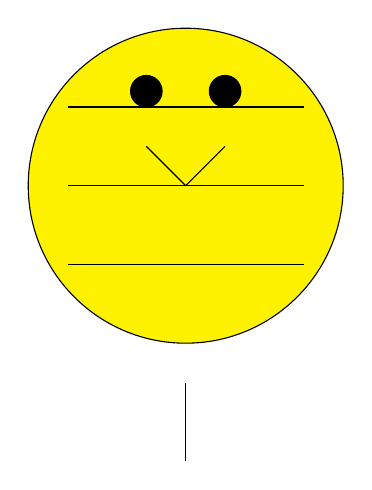
\begin{tikzpicture}
% Body
\draw [fill=yellow, draw=black] (0,0) circle (2);
% Horn
\draw [fill=white, draw=black] (0,0) -- (0.5,0.5);
\draw [fill=white, draw=black] (0,0) -- (-0.5,0.5);
% Legs
\draw [fill=black, draw=black] (-1.5,1) -- (1.5,1);
\draw [fill=black, draw=black] (-1.5,0) -- (1.5,0);
\draw [fill=black, draw=black] (-1.5,-1) -- (1.5,-1);
% Tail
\draw [fill=black, draw=black] (0,-2.5) -- (0,-3.5);
% Eyes
\draw [fill=black] (-0.5,1.2) circle (0.2);
\draw [fill=black] (0.5,1.2) circle (0.2);
\end{tikzpicture}

\subsection{Second}

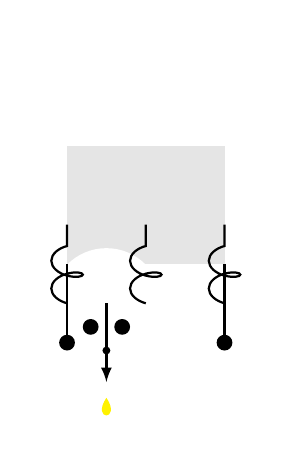
\begin{tikzpicture}
  % Body
  \fill[white] (0,0) circle (1.5);
  \fill[gray!20] (-1,-1.5) -- (1,-1.5) -- (1,0) -- (-1,0) -- cycle;
  
  % Neck and head
  \fill[white] (-0.5,-2) circle (0.7);
  \draw[-latex, thick] (-0.5,-2) -- (-0.5,-3);
  
  % Horn
  \fill[yellow] (-0.5,-3.2) .. controls (-0.7,-3.5) and (-0.3,-3.5) .. (-0.5,-3.2);
  
  % Eyes and nostrils
  \fill[black] (-0.7,-2.3) circle (0.1);
  \fill[black] (-0.3,-2.3) circle (0.1);
  \fill[black] (-0.5,-2.6) circle (0.05);
  
  % Mane
  \foreach \x in {-1,...,1} {
    \draw[thick, decorate, decoration={coil, amplitude=2mm}] (\x,-2) -- (\x,-1);
  }
  
  % Legs
  \foreach \x in {-1,1} {
    \draw[thick] (\x,-1.5) -- (\x,-2.5);
    \fill[black] (\x,-2.5) circle (0.1);
  }
\end{tikzpicture}

\section{Qwen1.5 110B-Chat-demo}
\subsection{First - 4/20/2024}
\begin{tikzpicture}[scale=1]

% Body
\draw (0,0) to [out=60,in=240] (2,2) -- (5,2) to [out=60,in=240] (7,4) -- (8,4);

% Legs
\draw (2,2) -- (2,0);
\draw (5,2) -- (5,0);
\draw (7,4) to [out=270,in=0] (6,3) to [out=180,in=270] (5,4);

% Head and neck
\draw (8,4) to [out=90,in=0] (7,5) to [out=180,in=90] (6,4);
\draw (6,4) to [out=-90,in=180] (7,3) to [out=0,in=-90] (8,4);

% Mane
\draw[decorate, decoration={zigzag,segment length=4,amplitude=1}] (6,5) -- (7,5);

% Tail
\draw[decorate, decoration={zigzag,segment length=4,amplitude=1}] (0,0) -- (-1,-1);

% Eye (simple representation)
\fill (6.5,4.2) circle (0.1);

% Horn
\draw (6,4) -- (5.5,3) -- (6,2);

\end{tikzpicture}

\subsection{Second - 4/20/2024}
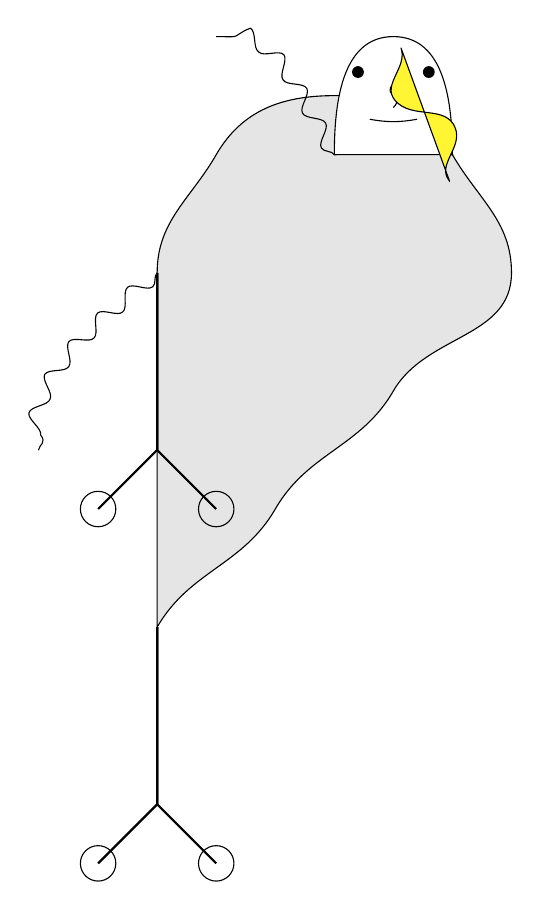
\begin{tikzpicture}[scale=1.5]
    % Body
    \draw[fill=gray!20] (0,0) to [out=60,in=240] (1,1) 
                          to [out=60,in=240] (2,2) 
                          to [out=60,in=270] (3,3)
                          to [out=90,in=300] (2.5,4)
                          to [out=120,in=0] (1.5,4.5)
                          to [out=180,in=60] (0.5,4)
                          to [out=240,in=90] (0,3)
                          to cycle;
    
    % Legs
    \draw[thick] (0,0) -- (0,-1.5) -- (-0.5,-2);
    \draw[thick] (0,0) -- (0,-1.5) -- (0.5,-2);
    \draw[thick] (0,3) -- (0,1.5) -- (-0.5,1);
    \draw[thick] (0,3) -- (0,1.5) -- (0.5,1);
    
    % Head
    \draw[fill=white] (2.5,4) to [out=90,in=0] (2,5) to [out=180,in=90] (1.5,4) to cycle;
    
    % Eyes
    \fill (1.7,4.7) circle (0.05);
    \fill (2.3,4.7) circle (0.05);
    
    % Nose
    \draw (2,4.6) .. controls (1.9,4.5) and (2.1,4.5) .. (2,4.4);
    
    % Mouth
    \draw (1.8,4.3) to [out=-10,in=190] (2.2,4.3);
    
    % Mane
    \draw[decorate,decoration={snake,amplitude=1mm,segment length=5mm}] (1.5,4) to [out=120,in=0] (0.5,5);
    
    % Tail
    \draw[decorate,decoration={snake,amplitude=1mm,segment length=5mm}] (0,3) to [out=220,in=90] (-1,1.5);
    
    % Horn
    \draw[fill=yellow!80!white,rotate around={20:(2.5,4)}] (2.4,3.8) to [out=110,in=-90] (2.6,4.2) to [out=90,in=-70] (2.2,4.6) to [out=110,in=-90] (2.4,5) to cycle;
    
    % Hooves
    \foreach \x in {-0.5,0.5} {
        \draw (\x,-2) circle (0.15);
        \draw (\x,1) circle (0.15);
    }
\end{tikzpicture}
\end{document}


